\documentclass[a4paper]{article}

% Importazioni
\usepackage{import}
% ----- Codifica, lingua, font -----
\usepackage[T1]{fontenc}
\usepackage[utf8]{inputenc}
\usepackage[italian]{babel}

% ----- Layout e impaginazione -----
\usepackage{geometry}
\geometry{a4paper, top=3cm, bottom=3cm, left=3cm, right=3cm}

\usepackage{titlesec}
\usepackage{fancyhdr}
\usepackage{graphicx}
\usepackage{float}
\usepackage{caption}
\usepackage{subcaption}
\setlength{\parindent}{0pt}

\usepackage{booktabs}
\usepackage{csquotes}
\usepackage[table]{xcolor}

% ----- Numerazione sezioni fino al 4° livello -----
\setcounter{secnumdepth}{5}
\setcounter{tocdepth}{5}

% ----- Sezione fino al 4° livello (subsubsubsection) -----
\newcounter{subsubsubsection}[subsubsection]
\renewcommand{\thesubsubsubsection}{\thesubsubsection.\arabic{subsubsubsection}}
\newcommand{\subsubsubsection}[1]{%
    \refstepcounter{subsubsubsection}%
    \addcontentsline{toc}{subparagraph}{\thesubsubsubsection\quad #1}%
    \vspace{1ex}\noindent\textbf{\thesubsubsubsection\quad #1}\par\nopagebreak\vspace{0.5ex}
}

% ----- Intestazione/Piè di pagina -----
\pagestyle{fancy}
\fancyhead[L]{\nouppercase{\leftmark}}
\fancyhead[R]{\nouppercase{\rightmark}}
\fancyfoot[C]{\thepage}

% ----- Stile titoli sezione -----
\titleformat{\section}
{\normalfont\Large\bfseries\centering}
{\makebox[0pt][r]{\textcolor{gray}{\fontsize{40}{40}\selectfont\thesection\hspace{0.3em}}}}
{0pt}
{\Huge}
[\vspace{1em}\titlerule]

\titlespacing*{\section}{0pt}{45pt}{20pt}

% Interruzione automatica prima di ogni sezione
\let\oldsection\section
\renewcommand\section{\newpage\oldsection}

% ----- Colori personalizzati -----
\definecolor{verde}{RGB}{0, 153, 0}
\arrayrulecolor[HTML]{808080}

% ----- Tipografia matematica -----
\usepackage{amsmath, amssymb, amsthm, mathtools}
\usepackage{mdframed}
\newmdtheoremenv{theo}{Teorema}

% ----- Codice e pseudocodice -----
\usepackage{listings}
\lstdefinelanguage{Pseudocode}{
    keywordstyle=\color{blue}\bfseries,
    keywords={if, else, while, for, function, return, end},
    ndkeywords={input, output, var},
    sensitive=false,
    comment=[l]{//},
    morecomment=[s]{/*}{*/},
    morestring=[b]",
    basicstyle=\ttfamily,
    stringstyle=\color{red},
    commentstyle=\color{green!60!black},
}
\lstdefinestyle{modern}{
    backgroundcolor=\color{blue!5},
    commentstyle=\color{gray!70},
    keywordstyle=\color{blue}\bfseries,
    stringstyle=\color{green!70},
    basicstyle=\ttfamily\small,
    numberstyle=\tiny\color{blue},
    numbers=left,
    stepnumber=1,
    frame=single,
    framesep=3pt,
    frameround=tttt,
    rulecolor=\color{blue!35},
    breakatwhitespace=false,
    tabsize=2,
    captionpos=b,
    escapeinside={(*@}{@*)},
    mathescape=true,
}

% ----- Grafici e figure -----
\usepackage{tikz}
\usetikzlibrary{shapes.misc}
\usepackage{pgfplots}
\pgfplotsset{compat=1.18}
\usepgfplotslibrary{fillbetween}
\usepackage{pgf-pie}

% ----- Citazioni, bibliografia, note -----
\usepackage{quoting}
\usepackage[
    backend=biber,
    style=alphabetic,
    sorting=ynt
]{biblatex}
\addbibresource{bibliografia.bib}

% ----- Hyperlink (nascosti ma attivi) -----
% Carica hyperref con le opzioni per i link interni (document links)
\usepackage{hyperref}
\hypersetup{
    colorlinks=true,  % Rende i link colorati anziché avere un bordo
    linkcolor=blue,   % Colore per i link interni (es. \ref, \autoref, \hyperlink)
    citecolor=green,  % Colore per le citazioni
    filecolor=magenta,
    urlcolor=cyan,
    pdftitle={Your Document Title}, % Aggiungi un titolo per il PDF
    pdfauthor={Your Name}, % Aggiungi l'autore del PDF
    pdfsubject={Your Subject}, % Aggiungi l'argomento del PDF
    pdfkeywords={Keyword1, Keyword2}, % Aggiungi parole chiave
}

% Ridefinisce \tableofcontents per avere link invisibili
\let\oldtableofcontents\tableofcontents
\renewcommand{\tableofcontents}{%
    \begingroup
    \hypersetup{linkcolor=black, hidelinks=true} % Nasconde i link solo per l'indice
    \oldtableofcontents
    \endgroup
}


% ----- Titolo con sottotitolo -----
\usepackage[cc]{titlepic}
\makeatletter
\providecommand{\subtitle}[1]{%
    \apptocmd{\@title}{\par {\large #1 \par}}{}{}
}
\makeatother

% ----- Spaziatura tabelle -----
\setlength{\arrayrulewidth}{0.3mm}
\setlength{\tabcolsep}{18pt}
\renewcommand{\arraystretch}{1.5}
\newcolumntype{s}{>{\columncolor[HTML]{FFFFFF}} p{3cm}}

% ----- Comandi personalizzati -----
\newcommand{\lapl}{\mathcal{L}}
\colorlet{stepnote}{black}
\newcommand{\stepnote}[1]{&&\text{\color{stepnote}#1}}

\begin{document}

% Titolo
\begin{titlepage}
    $ $
    \vspace{5pt}
    \newcommand{\HRule}{\rule{\linewidth}{0.5mm}}
    \begin{center}
    \textsc{\normalsize track tune}\\[1cm]
    %\text{\large Relazione conclusiva}\\[0.5cm] % Minor heading such as course title
    \end{center}
    
    \center
     
    %----------------------------------------------------------------------------------------
    %	HEADING SECTIONS
    %----------------------------------------------------------------------------------------
    
    \HRule \\[0.4cm]
    { \huge \bfseries SW Engineering Documentation}\\[0.4cm] % Title of your document
    \HRule \\[1.5cm]
     
    %----------------------------------------------------------------------------------------
    %	AUTHOR SECTION
    %----------------------------------------------------------------------------------------
    
    \begin{minipage}{0.4\textwidth}
    \begin{flushleft} \large
    \emph{Autori:}\\
    Mattia \textsc{Rebonato} \\
    Davide \textsc{Fozzato}\\
    \end{flushleft}
    \end{minipage}
    ~
    \begin{minipage}{0.4\textwidth}
    \begin{flushright} \large
    \emph{Professore:} \\
    Prof Carlo \textsc{Combi}
    \end{flushright}
    \end{minipage}\\[2cm]
    
    \vspace{250pt}
    
    \textsc{\normalsize A.A. 2024-2025}\\[0.5cm]
    
    \vfill % Fill the rest of the page with whitespace
    \end{titlepage}

\tableofcontents
\pagebreak

% =======================
\section{Introduzione}
% =======================

\subsection{Prefazione}

Il presente documento definisce in modo esaustivo i requisiti, l'architettura e le specifiche di progettazione del software \textit{TrackTune},
una piattaforma applicativa dedicata alla gestione, condivisione e analisi 
collaborativa di contenuti musicali.\\[2ex] 

La documentazione è rivolta a sviluppatori, tester, amministratori di sistema e a 
tutti gli stakeholder coinvolti nella realizzazione, manutenzione e gestione del 
progetto.

\subsection{Panoramica}

La piattaforma si rivolge a musicisti, compositori, insegnanti, studenti e appassionati
di musica, offrendo un ambiente digitale comodo per l’archiviazione, la collaborazione 
e l’accesso a materiale musicale di vario genere, tra cui spartiti, testi, accordi, 
file audio/video e link esterni (ad esempio YouTube).

Essa si propone non solo come archivio digitale, 
ma anche come spazio per l’approfondimento culturale, 
lo scambio di interpretazioni e feedback tra utenti, favorendo la condivisione 
di esperienze musicali, commenti critici e annotazioni esecutive su brani e 
contenuti attinenti alla musica.

% ==============================
\section{Analisi dei requisiti}
% ==============================

\subsection{Descrizione del sistema}

Si vuole progettare un sistema software per gestire la collezione e la condivisione 
di spartiti, testi, accordi, MIDI, MP3, video, link e molto altro, relativamente a brani 
musicali di diversa tipologia/genere.\\[2ex]

Gli utenti, previa autorizzazione dell'amministratore, devono poter caricare, 
scaricare, commentare e interagire con i vari contenuti. Per ogni risorsa il sistema deve
consentire di specificare:
\begin{itemize}
    \item autori
    \item genere/generi
    \item strumenti musicali utilizzati
\end{itemize}

Inoltre, per le risorse multimediali (audio, video, ecc.) il sistema deve
consentire di specificare il luogo e la data di registrazione.

Ogni utente può aggiungere note di testo libero su segmenti specifici di esecuzione (MP3, MP4 o video YouTube).  
Un segmento è definito dal momento di inizio e fine, e per ciascuno è possibile includere dettagli come assoli, esecutori, strumenti,
ritmi e altre caratteristiche. I commenti possono essere arricchiti con ulteriori 
risposte, consentendo una profondità illimitata di discussioni relativamente a quel 
contenuto.\\[2ex]

Un brano può essere inserito anche da un autore o un interprete. Deve essere possibile 
quindi distinguere il proprio ruolo all’interno del brano e, nel caso di interpreti, 
gli strumenti utilizzati. I commenti sulle modalità esecutive devono apparire in maniera 
rilevante rispetto a quelli di altri utenti.\\[2ex]

I video YouTube possono essere visualizzati direttamente nel software o nel browser, 
ma tutti i commenti relativi sono gestiti dal sistema.\\[2ex]

Gli utenti possono aggiungere commenti su spartiti, testi e accordi, 
relativi alle modalità esecutive (come strumenti, ritmo, intensità, ecc.), sia su 
specifiche parti del brano che sull'intero brano.\\[2ex]

Un utente può richiedere la registrazione alla piattaforma tramite un form, che 
l'amministratore valuterà e risponderà a seconda dell’esito.  
L'amministratore gestisce gli utenti, ha il compito di rimuovere coloro che pubblicano contenuti non pertinenti 
e di moderare i commenti. Inoltre, valuta le richieste di registrazione, il cui esito verrà comunicato 
all’utente interessato.\\[2ex]

Il sistema deve permettere la ricerca delle risorse tramite i seguenti filtri:
\begin{itemize}
    \item genere
    \item titolo del brano
    \item autore/i
\end{itemize}

Ogni risorsa per cui un utente ha lasciato un commento deve essere direttamente accessibile.

Gli strumenti musicali, i generi, i titoli dei brani e i nomi degli autori vanno gestiti attraverso dizionari aggiornabili, da usare anche per le opportune ricerche.

\subsection{Requisiti funzionali}

\subsubsection{Gestione degli utenti}
\begin{itemize}
    \item Registrazione tramite form dedicato;
    \item Valutazione da parte dell’amministratore delle richieste di registrazione e relativa comunicazione dell’esito;
    \item Profilazione (distinzione tra utente/amministratore);
    \item Autorizzazione al caricamento dei file per utente;
\end{itemize}

\subsubsection{Gestione dei contenuti}
\begin{itemize}
    \item Aggiunta, modifica e rimozione di contenuti multimediali
    \begin{itemize}
        \item La rimozione può essere eseguita solo dall’amministratore o dall’utente che ha caricato il contenuto
    \end{itemize}
    \item Visualizzazione delle risorse tramite software di terze parti o tramite l’applicativo stesso.
    \item Moderazione degli utenti
    \begin{itemize}
        \item L’amministratore può rimuovere utenti;
        \item L’amministratore può rimuovere commenti/risorse inappropriate.
    \end{itemize}
    \item Gestione dei dizionari aggiornabili (solo amministatore) relativi a:
    \begin{itemize}
        \item Autori;
        \item Generi;
        \item Strumenti musicali;
    \end{itemize}
\end{itemize}

\subsubsection{Gestione dei commenti}
\begin{itemize}
    \item Possibilità di commentare brani;
    \item Possibilità di rispondere ai commenti;
    \item Possibilità di commentare su specifici segmenti di esecuzione;
    \item Visualizzazione differenziata dei commenti per autori/esecutori del brano.
\end{itemize}

\subsection{Casi d'uso}
L’applicazione sarà disponibile esclusivamente agli utenti abilitati dall’amministratore, il quale è anch’esso un utente ma con privilegi di amministrazione sui comportamenti del sistema. L’unica operazione che può effettuare un utente non registrato è la richiesta di creazione di un account.

\begin{figure}[H]
    \centering
    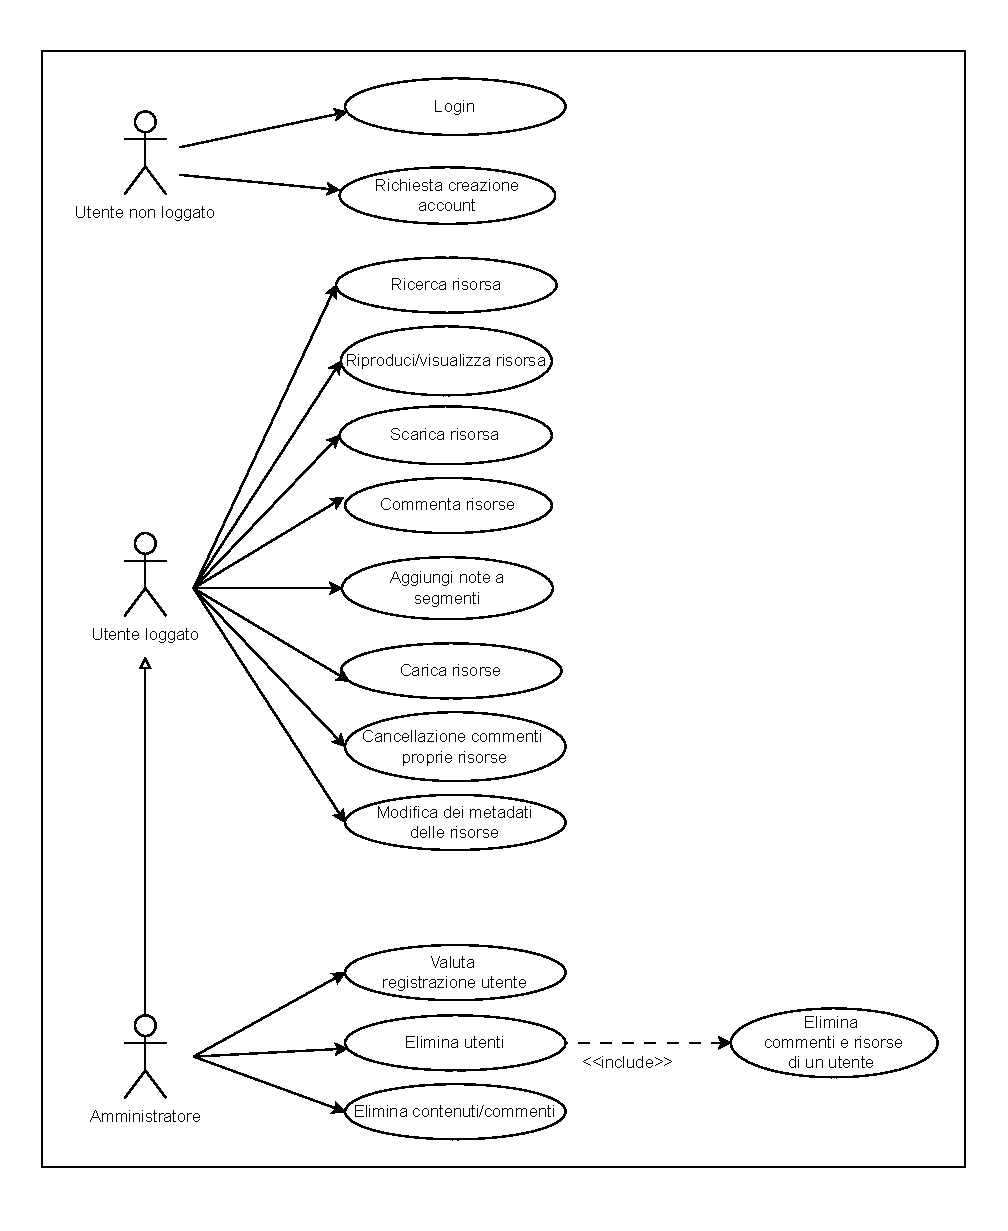
\includegraphics[width=0.8\textwidth]{./figures/use_cases}
    \caption{Use Cases}
    \label{fig:use_cases}
\end{figure}
\newpage
\subsubsection{Utente non loggato}
L'utente non autenticato può effettuare esclusivamente non operazioni:
    \begin{enumerate}
        \item Richiedere un account ad un amministratore
        \item Effettuare l'accesso tramite un form di autenticazione
    \end{enumerate}

\begin{table}[H]
\centering
\renewcommand{\arraystretch}{1.5}
\begin{tabular}{|>{\bfseries}l|p{10cm}|}
\hline
\multicolumn{2}{|c|}{\textbf{Caso d'uso: Login}} \\
\hline
\textbf{Id} & UC$0$ \\ \hline
\textbf{Attori} & Utente non loggato \\ \hline
\textbf{Precondizioni} & L’utente non è autenticato sulla piattaforma. \\ \hline
\textbf{Sequenza degli eventi} &
\begin{enumerate}
    \item L’utente compila i campi per effettuare l'autenticazione
    \item Il sistema verifica i dati e gestisce le autorizzazioni dell'utente
\end{enumerate}\\ \hline
\textbf{Post condizioni} & Utente autenticato e correttamente gestito \\ \hline
\end{tabular}
\caption{Descrizione caso d'uso \textit{Login}}
\label{tab:login-usecase}
\end{table}


\begin{table}[H]
    \centering
    \renewcommand{\arraystretch}{1.5}
    \begin{tabular}{|>{\bfseries}l|p{10cm}|}
        \hline
        \multicolumn{2}{|c|}{\textbf{Caso d'uso: Richiesta creazione account}} \\
        \hline
        \textbf{Id} & UC$1$ \\ \hline
        \textbf{Attori} & Utente non loggato \\ \hline
        \textbf{Precondizioni} & L’utente non è autenticato sulla piattaforma. \\
        & L’utente accede alla sezione di registrazione. \\ \hline % Added a new line and an empty cell for proper alignment
        \textbf{Sequenza degli eventi} &
        \begin{enumerate}
            \item Vengono compilati i dati relativi alla richiesta
            \item La richiesta viene inviata
            \item Il sistema registra la richiesta e la mette in stato di approvazione
            \item L'account viene salvato come account provvisorio e viene inserita una password temporanea
            \item Il sistema notifica l’amministratore della nuova richiesta
        \end{enumerate}\\ \hline
        \textbf{Sequenza alternativa } & Utente già esistente che comporta un messaggio di errore \\ \hline
        \textbf{Post condizioni} & La richiesta di creazione dell'account deve essere approvata da un amministratore \\ \hline
    \end{tabular}
    \caption{Descrizione caso d'uso \textit{Richiesta creazione account}}
    \label{tab:request_account-usecase}
\end{table}

\begin{figure}[H]
    \centering
    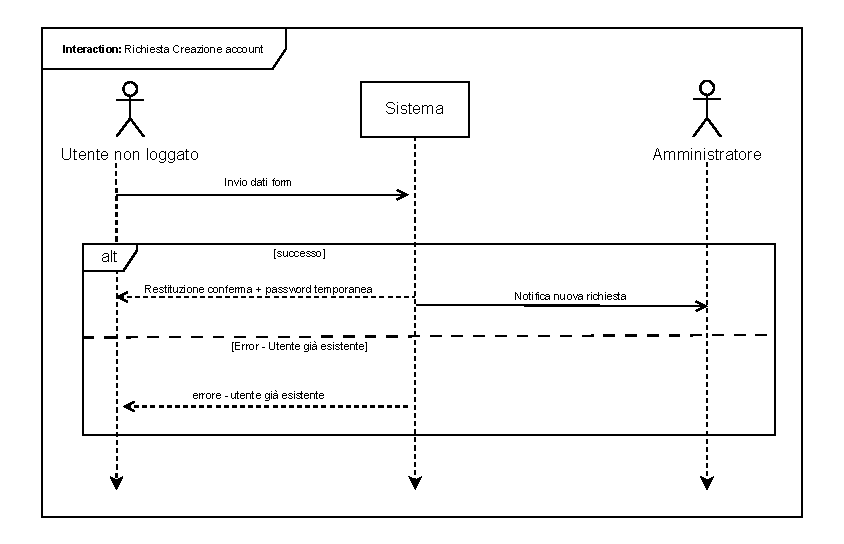
\includegraphics[width=0.9\textwidth]{./figures/account_request_sd}
    \caption{Sequence diagram del caso d'uso \textit{Richiesta creazione account}}
    \label{fig:sd_request_account}
\end{figure}
    
\subsubsection{Utente loggato}
\begin{table}[H]
    \centering
    \renewcommand{\arraystretch}{1.5}
    \begin{tabular}{|>{\bfseries}l|p{10cm}|}
        \hline
        \multicolumn{2}{|c|}{\textbf{Caso d'uso: Ricerca risorsa}} \\
        \hline
        \textbf{Id} & UC2 \\ \hline
        \textbf{Attori} & Utente loggato \\ \hline
        \textbf{Precondizioni} & Utente autenticato \\ \hline
        \textbf{Sequenza degli eventi} &
        \begin{enumerate}
            \item Il sistema invia i criteri di filtro disponibili
            \item L'utente decide il filtro di ricerca
            \item L'utente inserisce una parola chiave per ricercare una risorsa
            \item Gli vengono restituite le risorse data quella ricerca
        \end{enumerate}\\ \hline
        \textbf{Sequenza alternativa 1} & Errore nella ricerca: messaggio di errore \\ \hline
        \textbf{Post condizioni} & L'utente ha visualizzato la risorsa correttamente \\ \hline
    \end{tabular}
    \caption{Descrizione caso d'uso \textit{Ricerca risorsa}}
    \label{tab:search_resource-usecase}
\end{table}

\begin{figure}[H]
    \centering
    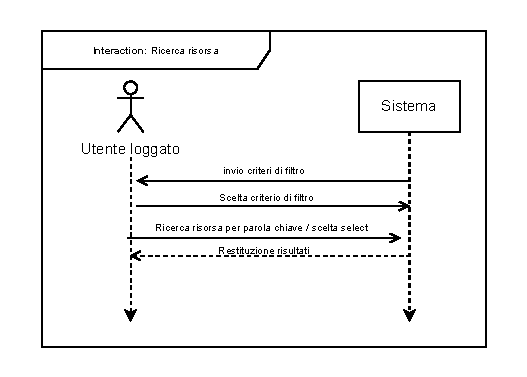
\includegraphics{./figures/ricerca_risorsa_sd}
    \caption{Sequence diagram del caso d'uso \textit{Ricerca risorsa}}
    \label{fig:sd_ricerca_risorsa}
\end{figure}

\begin{table}[H]
    \centering
    \renewcommand{\arraystretch}{1.5}
    \begin{tabular}{|>{\bfseries}l|p{10cm}|}
        \hline
        \multicolumn{2}{|c|}{\textbf{Caso d'uso: Riproduci/Visualizza risorsa}} \\
        \hline
        \textbf{Id} & UC3 \\ \hline
        \textbf{Attori} & User Logged \\ \hline
        \textbf{Precondizioni} &
        Utente autenticato \\& L'utente ha effettuato una ricerca o ne può selezionare una
        \\ \hline
        \textbf{Sequenza degli eventi} &
        \begin{enumerate}
            \item L'utente seleziona una risorsa dal risultato delle ricerca
            \item Il sistema riconosce il tipo di risorsa
            \item Se multimediale, lo riproduce
            \item Se testuale, lo visualizza
        \end{enumerate}\\ \hline
        \textbf{Sequenza alternativa 1} & Errore nella riproduzione: messaggio di errore \\ \hline
        \textbf{Post condizioni} & L'utente ha visualizzato la risorsa \\ \hline
    \end{tabular}
    \caption{Descrizione caso d'uso \textit{Riproduci/Visualizza risorsa}}
    \label{tab:play_view_resource-usecase}
\end{table}

\begin{figure}[H]
    \centering
    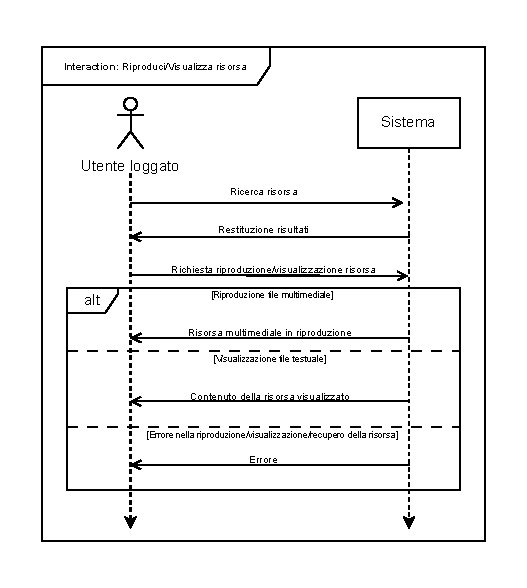
\includegraphics{./figures/visualizza_risorsa_sd}
    \caption{Sequence diagram del caso d'uso \textit{Riproduci/Visualizza risorsa}}
    \label{fig:sd_visualizza_risorsa}
\end{figure}

\begin{table}[H]
    \centering
    \renewcommand{\arraystretch}{1.5}
    \begin{tabular}{|>{\bfseries}l|p{10cm}|}
        \hline
        \multicolumn{2}{|c|}{\textbf{Caso d'uso: Scarica risorsa}} \\
        \hline
        \textbf{Id} & UC4 \\ \hline
        \textbf{Attori} & User Logged \\ \hline
        \textbf{Precondizioni} & Utente autenticato \\
        & L'utente ha effettuato una ricerca o ne può selezionare una \\ \hline
        \textbf{Sequenza degli eventi} &
        \begin{enumerate}
            \item L'utente seleziona una risorsa dal risultato delle ricerca
            \item L'utente richiede il download della risorsa
        \end{enumerate}\\ \hline
        \textbf{Sequenza alternativa 1} & Errore nel download: messaggio di errore \\ \hline
        \textbf{Post condizioni} & L'utente ha scaricato la risorsa correttamente \\ \hline
    \end{tabular}
    \caption{Descrizione caso d'uso \textit{Scarica risorsa}}
    \label{tab:download_resource-usecase}
\end{table}

\begin{figure}[H]
    \centering
    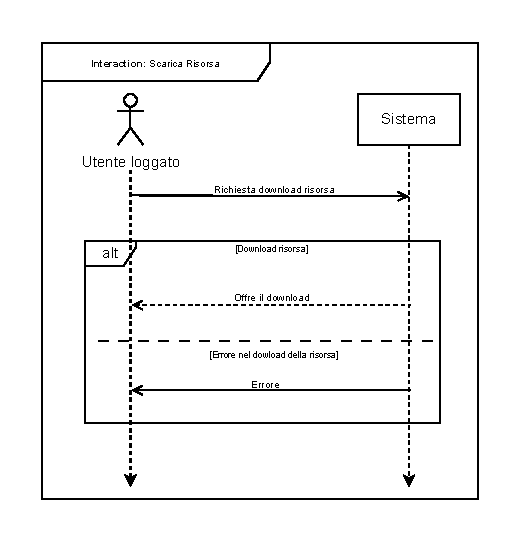
\includegraphics{./figures/scarica_sd}
    \caption{Sequence diagram del caso d'uso \textit{Scarica risorsa}}
    \label{fig:sd_download_resource}
\end{figure}

\begin{table}[H]
    \centering
    \renewcommand{\arraystretch}{1.5}
    \begin{tabular}{|>{\bfseries}l|p{10cm}|}
        \hline
        \multicolumn{2}{|c|}{\textbf{Caso d'uso: Commenta risorse}} \\
        \hline
        \textbf{Id} & UC5 \\ \hline
        \textbf{Attori} & User Logged \\ \hline
        \textbf{Precondizioni} & Utente autenticato \\
        & L'utente può visualizzare una risorsa \\ \hline
        \textbf{Sequenza degli eventi} &
        \begin{enumerate}
            \item L'utente seleziona una risorsa dal risultato delle ricerca
            \item L'utente può scrivere un commento
            \item Il commento viene salvato dal sistema
        \end{enumerate}\\ \hline
        \textbf{Sequenza alternativa 1} & L'utente può rispondere ad un commento \\ \hline
        \textbf{Post condizioni} & L'utente ha commentato la risorsa correttamente \\ \hline
    \end{tabular}
    \caption{Descrizione caso d'uso \textit{Commenta risorse}}
    \label{tab:comment_resource-usecase}
\end{table}

\begin{figure}[H]
    \centering
    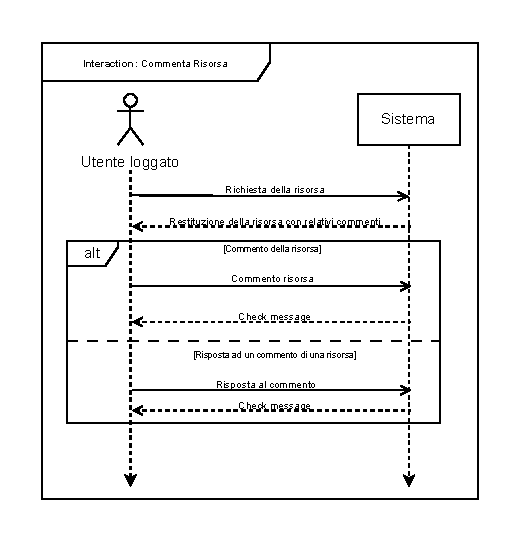
\includegraphics{./figures/commenta_risorsa_sd}
    \caption{Sequence diagram del caso d'uso \textit{Commenta risorse}}
    \label{fig:sd_commenta_risorsa}
\end{figure}

\begin{table}[H]
    \centering
    \renewcommand{\arraystretch}{1.5}
    \begin{tabular}{|>{\bfseries}l|p{10cm}|}
        \hline
        \multicolumn{2}{|c|}{\textbf{Caso d'uso: Aggiungi note a segmenti}} \\
        \hline
        \textbf{Id} & UC6 \\ \hline
        \textbf{Attori} & User Logged \\ \hline
        \textbf{Precondizioni} & Utente autenticato \\
        & L'utente ha ricercato/può visualizzare una risorsa \\ \hline
        \textbf{Sequenza degli eventi} &
        \begin{enumerate}
            \item L'utente seleziona un intervallo di tempo per inserire una nota/commento
            \item Scrive la /commento desiderata
            \item Invia la nota/commento al sistema
            \item Il sistema registra la nota/commento
        \end{enumerate}\\ \hline
        \textbf{Post condizioni} & L'utente ha scritto una nota/commento su un segmento correttamente \\ \hline
    \end{tabular}
    \caption{Descrizione caso d'uso \textit{Aggiungi note a segmenti}}
    \label{tab:add_notes_to_segments-usecase}
\end{table}


\begin{table}[H]
    \centering
    \renewcommand{\arraystretch}{1.5}
    \begin{tabular}{|>{\bfseries}l|p{10cm}|}
        \hline
        \multicolumn{2}{|c|}{\textbf{Caso d'uso: Carica Risorse}} \\
        \hline
        \textbf{Id} & UC7 \\ \hline
        \textbf{Attori} & User Logged \\ \hline
        \textbf{Precondizioni} & Utente autenticato \\ \hline
        \textbf{Sequenza degli eventi} &
        \begin{enumerate}
            \item L'utente visualizza la schermata di upload dei file
            \item Seleziona la risorsa da caricare
            \item Inserisce i dati (file + metadati obbligatori)
            \item Invia i dati al sistema
            \item Il sistema li memorizza
        \end{enumerate}\\ \hline
        \textbf{Sequenza alternativa 1} & Errore di sistema: messaggio di errore \\ \hline
        \textbf{Sequenza alternativa 2} & Errore nell'inserimento dei dati: messaggio di errore \\ \hline
        \textbf{Post condizioni} & L'utente ha caricato la risorsa correttamente \\ \hline
    \end{tabular}
    \caption{Descrizione caso d'uso \textit{Carica Risorse}}
    \label{tab:upload_resources-usecase}
\end{table}

\begin{figure}[H]
    \centering
    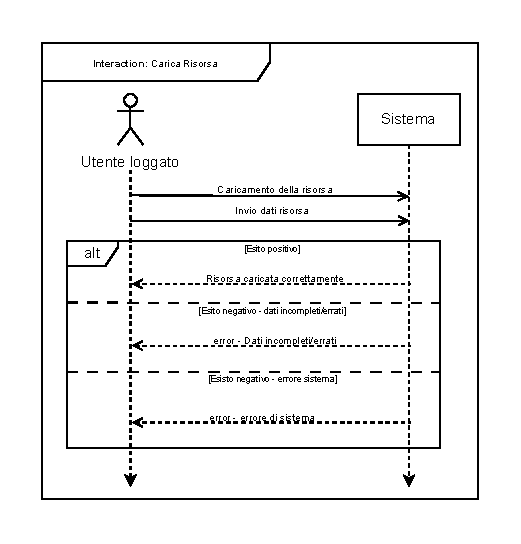
\includegraphics{./figures/carica_risorsa_sd}
    \caption{Sequence diagram del caso d'uso \textit{Carica Risorse}}
    \label{fig:sd_carica_risorsa}
\end{figure}

\begin{table}[H]
    \centering
    \renewcommand{\arraystretch}{1.5}
    \begin{tabular}{|>{\bfseries}l|p{10cm}|}
        \hline
        \multicolumn{2}{|c|}{\textbf{Caso d'uso: Cancellazione commenti delle proprie risorse}} \\
        \hline
        \textbf{Id} & UC8 \\ \hline
        \textbf{Attori} & User Logged \\ \hline
        \textbf{Precondizioni} & Utente autenticato e autorizzato \\
        & L'utente sta visualizzando una propria risorsa caricata \\ \hline
        \textbf{Sequenza degli eventi} &
        \begin{enumerate}
            \item L'utente desidera eliminare un qualsiasi commento della risorsa
            \item Elimina il commento
            \item Il sistema controlla che abbia i permessi necessari
            \item In caso positivo effettua la rimozione
            \item Vengono rimossi tutte le risposte a quel commento
        \end{enumerate}\\ \hline
        \textbf{Sequenza alternativa 1} & Errore Autorizzazioni: messaggio di errore \\ \hline
        \textbf{Post condizioni} & L'utente ha eliminato il commento correttamente \\ \hline
    \end{tabular}
    \caption{Descrizione caso d'uso \textit{Cancellazione commenti delle proprie risorse}}
    \label{tab:delete_comments_own_resources-usecase}
\end{table}

\begin{table}[H]
    \centering
    \renewcommand{\arraystretch}{1.5}
    \begin{tabular}{|>{\bfseries}l|p{10cm}|}
        \hline
        \multicolumn{2}{|c|}{\textbf{Caso d'uso: Modifica dei metadati delle risorse}} \\
        \hline
        \textbf{Id} & UC9 \\ \hline
        \textbf{Attori} & User Logged Authorized \\ \hline
        \textbf{Precondizioni} & Utente autenticato \\
        & L'utente è il proprietario di quella risorsa \\
        & L'utente sta visualizzando i dati di una risorsa \\ \hline
        \textbf{Sequenza degli eventi} &
        \begin{enumerate}
            \item L'utente desidera modificare un qualsiasi metadato della risorsa
            \item Modifica i metadati
            \item Invia le modifiche al sistema
            \item Il sistema effettua la modifica
        \end{enumerate}\\ \hline
        \textbf{Post condizioni} & L'utente ha modificato correttamente i metadati di una risorsa \\ \hline
    \end{tabular}
    \caption{Descrizione caso d'uso \textit{Modifica dei metadati delle risorse}}
    \label{tab:modify_metadata_uc9-usecase}
\end{table}

    \subsubsection{Amministratore}
\begin{table}[H]
    \centering
    \renewcommand{\arraystretch}{1.5}
    \begin{tabular}{|>{\bfseries}l|p{10cm}|}
        \hline
        \multicolumn{2}{|c|}{\textbf{Caso d'uso: Valuta registrazione utente}} \\
        \hline
        \textbf{Id} & UC10 \\ \hline
        \textbf{Attori} & Administrator \\ \hline
        \textbf{Precondizioni} & L'amministratore accede alla sezione di gestione delle registrazioni utente in attesa di valutazione \\ \hline
        \textbf{Sequenza degli eventi} &
        \begin{enumerate}
            \item L'amministratore visualizza i dettagli
            \item L'amministratore approva/rifiuta la richiesta
            \item Il sistema elimina la richiesta e in caso di approvazione crea l'account
            \item Il sistema notifica all'utente l'esito
        \end{enumerate}\\ \hline
        \textbf{Post condizioni} & L'utente è registrato e abilitato all'accesso al sistema (se approvato) o la sua richiesta di registrazione viene rifiutata \\ \hline
    \end{tabular}
    \caption{Descrizione caso d'uso \textit{Valuta registrazione utente}}
    \label{tab:evaluate_user_registration-usecase}
\end{table}

\begin{figure}[H]
    \centering
    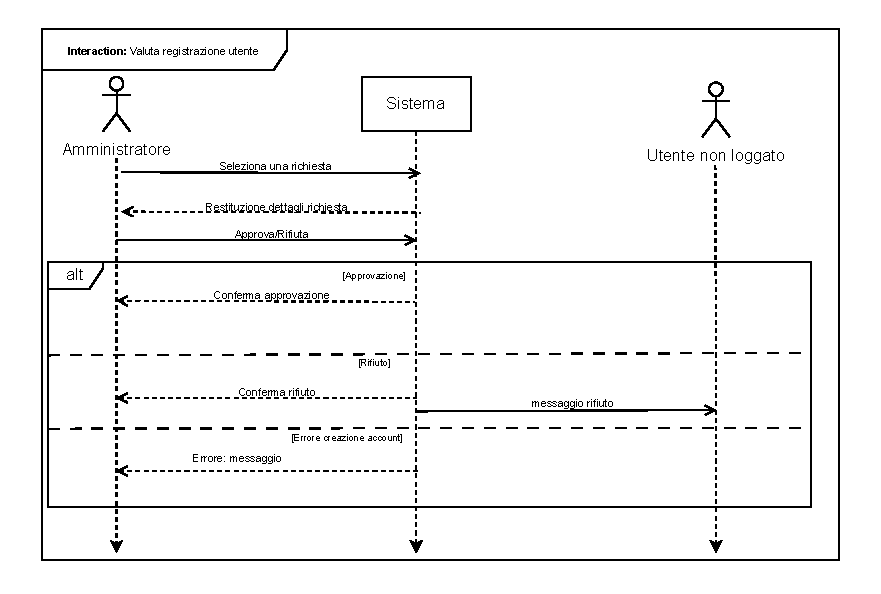
\includegraphics{./figures/valuta_richieste}
    \caption{Sequence diagram del caso d'uso \textit{Valuta registrazione utente}}
    \label{fig:sd_valuta_richiesta}
\end{figure}

\begin{table}[H]
    \centering
    \renewcommand{\arraystretch}{1.5}
    \begin{tabular}{|>{\bfseries}l|p{10cm}|}
        \hline
        \multicolumn{2}{|c|}{\textbf{Caso d'uso: Eliminazione utente}} \\
        \hline
        \textbf{Id} & UC11 \\ \hline
        \textbf{Attori} & Administrator \\ \hline
        \textbf{Precondizioni} & L'amministratore accede alla sezione di gestione degli utenti \\ \hline
        \textbf{Sequenza degli eventi} &
        \begin{enumerate}
            \item L'amministratore seleziona l'utente che desidera eliminare
            \item L'amministratore elimina l'utente
            \item Rimuove l'utente
        \end{enumerate}\\ \hline
        \textbf{Post condizioni} & L'utente è stato cancellato correttamente \\ \hline
    \end{tabular}
    \caption{Descrizione caso d'uso \textit{Eliminazione utente}}
    \label{tab:delete_user-usecase}
\end{table}

\begin{table}[H]
    \centering
    \renewcommand{\arraystretch}{1.5}
    \begin{tabular}{|>{\bfseries}l|p{10cm}|}
        \hline
        \multicolumn{2}{|c|}{\textbf{Caso d'uso: Elimina commenti e risorse di un utente}} \\
        \hline
        \textbf{Id} & UC12 \\ \hline
        \textbf{Attori} & Administrator \\ \hline
        \textbf{Precondizioni} & Caso d'uso \textit{Eliminazine Utente} (\autoref{tab:delete_user-usecase}) \\ \hline
        \textbf{Sequenza degli eventi} &
        \begin{enumerate}
            \item L'amministratore comunica al server un utente
            \item Le risorse e commenti di questo utente vengono eliminate
        \end{enumerate}\\ \hline
        \textbf{Post condizioni} & Le risorse/commenti sono stati cancellati correttamente \\ \hline
    \end{tabular}
    \caption{Descrizione caso d'uso \textit{Elimina commenti e risorse di un utente}}
    \label{tab:delete_user_comments_resources-usecase}
\end{table}

\begin{table}[H]
    \centering
    \renewcommand{\arraystretch}{1.5}
    \begin{tabular}{|>{\bfseries}l|p{10cm}|}
        \hline
        \multicolumn{2}{|c|}{\textbf{Caso d'uso: Elimina contenuti/commenti}} \\
        \hline
        \textbf{Id} & UC13 \\ \hline
        \textbf{Attori} & Administrator \\ \hline
        \textbf{Precondizioni} & Visualizzazione di una risorsa/commento \\ \hline
        \textbf{Sequenza degli eventi} &
        \begin{enumerate}
            \item L'amministratore visualizza una risorsa
            \item L'amministratore decide di eliminare la risorsa/commento
            \item Invia la richiesta al sistema
            \item Il sistema elimina la risorsa/commento
        \end{enumerate}\\ \hline
        \textbf{Post condizioni} & La risorsa/commento è stata eliminata correttamente \\ \hline
    \end{tabular}
    \caption{Descrizione caso d'uso \textit{Elimina contenuti/commenti}}
    \label{tab:delete_content_comments-usecase}
\end{table}


\subsection{Glossario dei termini}

\begin{table}[H]
    \centering
    \renewcommand{\arraystretch}{1.5}
    % Modifica qui:
    % Ad esempio, la prima colonna l'ho fatta p{0.25\textwidth}
    % e la seconda p{0.65\textwidth}. La somma (0.25+0.65=0.90) lascia spazio per i bordi e tabcolsep.
    \begin{tabular}{|>{\bfseries}p{0.28\textwidth}|p{0.62\textwidth}|}
        \hline
        \multicolumn{2}{|c|}{\textbf{GLOSSARIO DEI TERMINI}} \\
        \hline
        \textbf{TERMINE} & \textbf{DEFINIZIONE} \\
        \hline
        Contenuto musicale / Risorsa multimediale & Qualsiasi tipo di file audio, video o immagine caricato e reso disponibile sulla piattaforma. Può includere brani musicali, podcast, lezioni, video, ecc. \\
        \hline
        Autore / Esecutore / Interprete di un brano & L'individuo o il gruppo che ha contribuito in modo significativo alla creazione, composizione, esecuzione o interpretazione originale di un'opera musicale. \\
        \hline
        Segmento di un brano & Un sottoinsieme specifico di un contenuto multimediale (es. un brano musicale o un video), definito da un intervallo di tempo di inizio e fine, permettendo di focalizzare l'attenzione su una parte specifica. \\
        \hline
        Traccia & FOZZI SPIEGA TE BENE COSA INTENDI COSI SIAMO APPOSTO \\
        \hline
        Brano & Un'opera musicale originale completa e autonoma, che può essere parte di un album o una singola traccia, caratterizzata da una composizione unica. \\
        \hline
        Metadato & Un insieme di dati che descrivono e forniscono informazioni su altri dati (una risorsa). Per un brano, i metadati possono includere titolo, autore, genere, durata, data di pubblicazione, ecc. \\
        \hline
        Utente autenticato / Loggato & Un utente che ha completato con successo il processo di login fornendo credenziali valide ed è riconosciuto dal sistema, avendo accesso a funzionalità riservate. \\
        \hline
        Amministratore & Un utente con privilegi speciali all'interno della piattaforma, in grado di gestire utenti, contenuti, approvare richieste e monitorare le operazioni del sistema. \\
        \hline
        Richiesta di creazione account & La procedura iniziata da un utente non autenticato per ottenere un nuovo account sulla piattaforma, soggetta ad approvazione da parte di un amministratore. \\
        \hline
        Commento & Un testo o una nota aggiunta da un utente autenticato a una risorsa (o a un altro commento) per esprimere un'opinione, fornire feedback o interagire con altri utenti. \\
        \hline
        Nota a segmento & Un tipo specifico di commento o annotazione testuale associata a un intervallo di tempo preciso all'interno di una risorsa multimediale, permettendo di evidenziare o commentare una parte specifica del contenuto. \\
        \hline
    \end{tabular}
    \caption{Glossario dei Termini}
    \label{tab:glossary}
\end{table}

\subsection{Activity Diagrams}
Questa sezione illustra i principali flussi di lavoro del sistema attraverso gli activity diagrams.


% =======================
\section{Developing}
% =======================

\end{document}
